\documentclass[conference]{IEEEtran}

\usepackage{amsmath}
\usepackage{graphicx}
\usepackage{booktabs}
\usepackage{multirow}
\usepackage{tabularx}
\usepackage{tikz}
\usepackage{pgfplots}
\usepackage{placeins}
\usepackage{float}
\pgfplotsset{compat=1.18}
\usetikzlibrary{arrows.meta, positioning, shapes.geometric}

\title{Latency Side-Channel Fingerprinting of Neural Network Architectures via Inference Timing Analysis}

\author{
\IEEEauthorblockN{Shlok Pandey}
\IEEEauthorblockA{
Manipal Jaipur University \\
Email: shlokpandey8219@gmail.com
}
}

\begin{document}

\raggedbottom

\maketitle

% ---------------- ABSTRACT ----------------
\begin{abstract}
Latency-based side-channel leakage has emerged as a potential security risk in modern machine learning deployment environments. This paper investigates whether inference latency can be exploited to fingerprint neural network architectures in black-box settings. Different architectures, including VGG, ResNet, and Inception, exhibit distinct computational graph structures that influence inference timing behavior. The proposed methodology evaluates inference latency under controlled experimental conditions and extracts statistical timing features such as mean latency, standard deviation, and tail latency. These features are subsequently used for architecture classification using lightweight machine learning classifiers. Experimental results demonstrate that different architectures produce distinguishable timing signatures, enabling high-accuracy architecture identification using latency information alone. The findings highlight the security implications of timing leakage in machine learning systems and demonstrate that inference latency can act as a practical side-channel for neural network fingerprinting in cloud-based deployment settings.
\end{abstract}

% ---------------- INTRODUCTION ----------------
\section{Introduction}

Most cloud platforms and machine learning services provide hosted models through API-based interfaces. These services allow the user to query the system and get outputs. They often run in a black-box environment where the user has no visibility into the internal architecture. While this abstraction greatly improves usability and user access while protecting intellectual property, it also introduces potential security risks. In particular, systems may unintentionally leak information through side channels such as inference latency, power usage, memory/cache behavior, CPU/GPU utilization, packet sizes, and response sizes.

In this academic work, we focus specifically on inference latency. We methodically investigate whether the response time of neural network inference can reveal structural information about the underlying model, which can later possibly be used to create surrogate models.

We hypothesize that differences in the computational graph structures across architectures like VGG, ResNet, and Inception can leak distinct latency signatures that can be exploited for model fingerprinting.

% ---------------- BACKGROUND ----------------
\section{Background}

\subsection{Directed Acyclic Graphs (DAGs)}

A Directed Acyclic Graph (DAG) is a directed graph that does not contain any cycles. This graph consists of directed edges, and they signify a one-way relationship or dependency between nodes. 
The term ``acyclic'' indicates that there are no cycles or any closed loops within the graph, i.e., the user cannot traverse a sequence of directed edges and return to the same node while following edge directions. 

Modern neural network architectures can be modeled as DAGs, where the execution flow propagates through interconnected computational layers. Different neural network architectures exhibit different DAG structures. Sequential models such as VGG primarily show a linear computational graph, whereas architectures such as ResNet and Inception exhibit branching, merging, and parallel execution as they operate on the principles of skip connections and multi-scale feature extraction. These core structural differences alter the execution traits of the model, including inference latency, synchronization overhead, and computational variability. Consequently, DAG topology becomes an important factor in understanding latency-based side-channel behavior in neural network systems.

\subsection{Neural Network Architectures}

Neural network architectures vary significantly in their computational structure, execution flow, and layer organization. These differences in the architecture influence both model performance and inference characteristics. 

Sequential models such as VGG are characterized by their depth. VGG has deep stacks of convolutional layers arranged in a linear manner in a straightforward execution graph with minimal branching. Due to this highly sequential structure, inference propagates through a long chain of dependent operations.

\begin{figure}[!t]
\centering
\resizebox{\columnwidth}{!}{
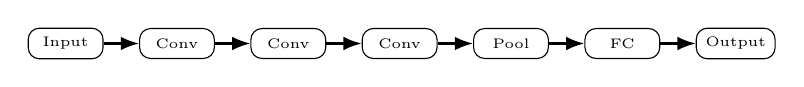
\begin{tikzpicture}[
    node distance=0.45cm,
    block/.style={draw, rounded corners, minimum width=0.95cm, minimum height=0.38cm, align=center, font=\tiny},
    arrow/.style={-{Latex}, thick}
]
\node[block] (input) {Input};
\node[block, right=of input] (conv1) {Conv};
\node[block, right=of conv1] (conv2) {Conv};
\node[block, right=of conv2] (conv3) {Conv};
\node[block, right=of conv3] (pool) {Pool};
\node[block, right=of pool] (fc) {FC};
\node[block, right=of fc] (out) {Output};

\draw[arrow] (input) -- (conv1);
\draw[arrow] (conv1) -- (conv2);
\draw[arrow] (conv2) -- (conv3);
\draw[arrow] (conv3) -- (pool);
\draw[arrow] (pool) -- (fc);
\draw[arrow] (fc) -- (out);
\end{tikzpicture}
}
\caption{Simplified VGG-style sequential computation graph.}
\label{fig:vgg}
\end{figure}

In contrast, architectures like ResNet are not just one single layer like VGG; they introduce a stack of repeating residual blocks connected through skip connections, which produce a branch-and-merge computation graph, allowing information to bypass intermediate layers. Consequently, the execution flow is no longer strictly sequential, producing a more complex Directed Acyclic Graph (DAG) structure compared to VGG.

\begin{figure}[!t]
\centering
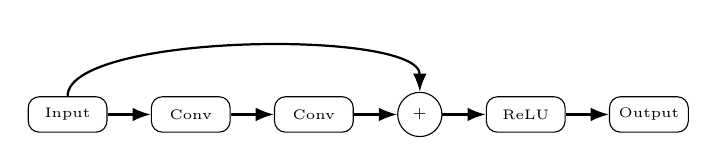
\begin{tikzpicture}[
    node distance=0.55cm,
    block/.style={draw, rounded corners, minimum width=1.0cm, minimum height=0.45cm, align=center, font=\tiny},
    add/.style={draw, circle, minimum size=0.35cm, font=\tiny},
    arrow/.style={-{Latex}, thick}
]
\node[block] (input) {Input};
\node[block, right=of input] (conv1) {Conv};
\node[block, right=of conv1] (conv2) {Conv};
\node[add, right=of conv2] (add) {$+$};
\node[block, right=of add] (relu) {ReLU};
\node[block, right=of relu] (out) {Output};

\draw[arrow] (input) -- (conv1);
\draw[arrow] (conv1) -- (conv2);
\draw[arrow] (conv2) -- (add);
\draw[arrow] (add) -- (relu);
\draw[arrow] (relu) -- (out);

\draw[arrow] (input.north) .. controls +(0,0.8) and +(0,0.8) .. (add.north);
\end{tikzpicture}
\caption{Simplified ResNet residual block with skip connection and merge operation.}
\label{fig:resnet}
\end{figure}

Early architectures, like VGG, mainly got better by increasing network depth. However, increasing network depth made computation expensive. The core idea for architectures like InceptionV3 was to increase representational power without increasing computation cost by executing a module that does multi-scale feature extraction efficiently. Instead of implementing one convolution choice at a layer, i.e., a single convolutional operation, the Inception module does multiple operations in parallel on the same input, then combines them. This produces wide branching inside each module and a concatenation merge, which results in a highly parallel DAG structure.

\begin{figure}[!t]
\centering
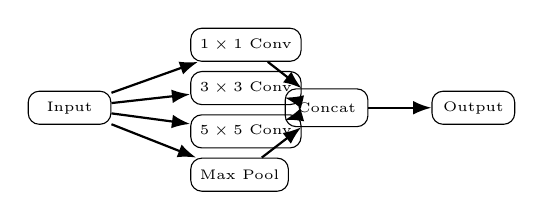
\begin{tikzpicture}[
    node distance=0.45cm,
    block/.style={draw, rounded corners, minimum width=1.05cm, minimum height=0.42cm, align=center, font=\tiny},
    concat/.style={draw, rounded corners, minimum width=1.05cm, minimum height=0.48cm, align=center, font=\tiny},
    arrow/.style={-{Latex}, thick}
]
\node[block] (input) {Input};

\node[block, right=1.0cm of input, yshift=0.8cm] (b1) {$1\times1$ Conv};
\node[block, right=1.0cm of input, yshift=0.25cm] (b2) {$3\times3$ Conv};
\node[block, right=1.0cm of input, yshift=-0.3cm] (b3) {$5\times5$ Conv};
\node[block, right=1.0cm of input, yshift=-0.85cm] (b4) {Max Pool};

\node[concat, right=2.2cm of input] (concat) {Concat};
\node[block, right=0.8cm of concat] (out) {Output};

\draw[arrow] (input) -- (b1);
\draw[arrow] (input) -- (b2);
\draw[arrow] (input) -- (b3);
\draw[arrow] (input) -- (b4);

\draw[arrow] (b1) -- (concat);
\draw[arrow] (b2) -- (concat);
\draw[arrow] (b3) -- (concat);
\draw[arrow] (b4) -- (concat);

\draw[arrow] (concat) -- (out);
\end{tikzpicture}
\caption{Simplified Inception-style multi-branch module with concatenation merge.}
\label{fig:inception}
\end{figure}

\subsection{Side-Channel Attacks}

A side-channel attack is a method of extracting information from a system without compromising the primary algorithm directly. Instead of exploiting the model parameters, such as CNN weights or encryption keys, the attacker observes the execution byproducts and indirect signals produced while the system operates.
Rather than targeting model parameters or architecture explicitly, side-channel attacks exploit observable characteristics like power consumption, memory access patterns, cache behavior, packet sizes, or inference latency.

Inference latency represents one of the most examinable and practical side channels in modern machine learning systems. Different neural network architectures demonstrate distinct execution characteristics during inference due to variations in computational graph topology, synchronization behavior, branching patterns, and computational complexity. These factors influence multiple stages of execution, including preprocessing overhead, model computation time, and post-processing latency.

As a result, different architectures produce distinct latency distributions during inference. In black-box deployment settings, an adversary may repeatedly query the model and analyze these timing variations to infer structural information about the underlying architecture.

\subsection{Black-Box Setting}

The experiment presumes a black-box deployment environment in which the attacker has no visibility into the internal architecture, parameters, data used in training, or implementation insights of the deployed neural network model. The target is accessible solely through a request-response interface. Despite complete restriction from internal access, the adversary can repeatedly query the model and observe inference response times. These timing records are further analyzed in order to infer structural characteristics of the underlying model.

% ---------------- THREAT MODEL ----------------
\section{Threat Model}

The threat model utilized in this work presumes an adversary engaging with a remotely hosted neural network system through an API interface. The attacker does not possess any information regarding internal mechanics, architecture, model weights, training dataset, hardware specifics, or implementation details of the deployed architecture.

However, the attacker is sufficiently capable of repeatedly requesting the target system and recording inference response times with high accuracy. By observing latency behavior across multiple readings, the attacker attempts to deduce structural properties of the underlying neural network. The main objective of the adversary is to perform architecture fingerprinting using latency-derived features in a black-box deployment environment.

% ---------------- METHODOLOGY ----------------
\section{Methodology}

\subsection{Model Selection}

For the purpose of this academic research, four convolutional neural network (CNN) architectures were selected: 

\begin{itemize}
    \item ResNet-18
    \item ResNet-50
    \item VGG-16
    \item InceptionV3
\end{itemize}

These models were loaded from \texttt{torchvision.models} and were selected because they represent significantly different computation graph structures. The first model, VGG, primarily follows a sequential structure, whereas ResNet introduces skip connections and residual blocks that create branch-and-merge computation paths. InceptionV3 further uses parallel branches and concatenation, increasing the structural complexity.

These architectural differences make the selected models suitable for evaluating whether computational graph structure influences inference latency and timing behavior.

\subsection{Latency Measurement}

Inference latency measurements were conducted on a Ryzen-7 based system using PyTorch. All models received identical input tensors of size \texttt{(1,3,224,224)} to ensure consistent evaluation conditions. Each model was switched to evaluation mode using \texttt{model.eval()} in order to disable training-specific behavior during inference. In addition, \texttt{torch.no\_grad()} was utilized to disable gradient computation and reduce unnecessary overhead during latency measurement. A warm-up inference pass was executed prior to timing measurements to reduce initialization overhead.

Each architecture executed 100 inference cycles, with individual inference times recorded using \texttt{time.perf\_counter()}. The duration of every forward pass was measured in milliseconds, producing a latency distribution for each architecture. Statistical features including mean latency, standard deviation, minimum latency, maximum latency, and P95 latency were subsequently extracted from these distributions. Figure~\ref{fig:latency_pipeline} illustrates the latency measurement workflow utilized during the experiments.

\begin{figure}[!t]
\centering
\resizebox{\columnwidth}{!}{
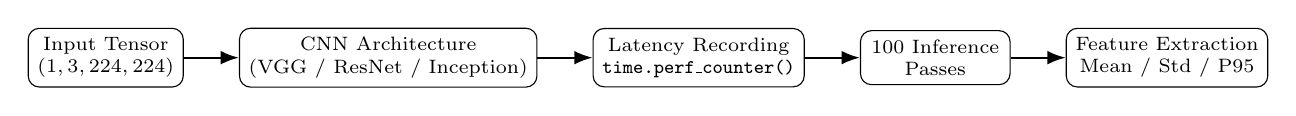
\begin{tikzpicture}[
    node distance=0.7cm,
    block/.style={
        draw,
        rounded corners,
        minimum width=1.9cm,
        minimum height=0.6cm,
        align=center,
        font=\scriptsize
    },
    arrow/.style={-{Latex}, thick}
]
\node[block] (input) {Input Tensor \\ $(1,3,224,224)$};
\node[block, right=of input] (model) {CNN Architecture \\ (VGG / ResNet / Inception)};
\node[block, right=of model] (timer) {Latency Recording \\ \texttt{time.perf\_counter()}};
\node[block, right=of timer] (repeat) {100 Inference \\ Passes};
\node[block, right=of repeat] (stats) {Feature Extraction \\ Mean / Std / P95};

\draw[arrow] (input) -- (model);
\draw[arrow] (model) -- (timer);
\draw[arrow] (timer) -- (repeat);
\draw[arrow] (repeat) -- (stats);
\end{tikzpicture}
}
\caption{Latency measurement and feature extraction pipeline utilized during inference experiments.}
\label{fig:latency_pipeline}
\end{figure}



\subsection{Feature Extraction}

Raw latency measurements were transformed into statistical timing features for architecture fingerprint generation. Instead of relying on individual latency observations, the proposed methodology summarized inference behavior using statistical descriptors including mean latency, standard deviation, minimum latency, maximum latency, and P95 latency. These features were selected because they capture both average execution behavior and latency variability across different neural network architectures.

Latency measurements were grouped across multiple inference queries in order to generate stable feature representations for classification. The resulting statistical feature vectors were subsequently associated with their corresponding architecture labels and used for downstream classification tasks.

Figure~\ref{fig:feature_pipeline} illustrates the statistical feature extraction pipeline utilized throughout the experiments.

\begin{figure}[!t]
\centering
\resizebox{\columnwidth}{!}{
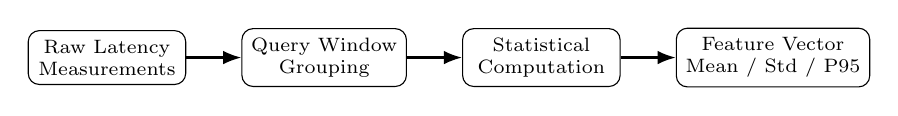
\begin{tikzpicture}[
    node distance=0.7cm,
    block/.style={
        draw,
        rounded corners,
        minimum width=2cm,
        minimum height=0.6cm,
        align=center,
        font=\scriptsize
    },
    arrow/.style={-{Latex}, thick}
]
\node[block] (latency) {Raw Latency \\ Measurements};
\node[block, right=of latency] (window) {Query Window \\ Grouping};
\node[block, right=of window] (stats) {Statistical \\ Computation};
\node[block, right=of stats] (feature) {Feature Vector \\ Mean / Std / P95};

\draw[arrow] (latency) -- (window);
\draw[arrow] (window) -- (stats);
\draw[arrow] (stats) -- (feature);
\end{tikzpicture}
}
\caption{Statistical feature extraction pipeline used for latency fingerprint generation.}
\label{fig:feature_pipeline}
\end{figure}



\subsection{Classification Approach}
Latency-derived feature vectors were used to train lightweight architecture classification models. Each feature vector represented the statistical timing characteristics of a specific neural network architecture including ResNet-18, ResNet-50, VGG-16, and InceptionV3.

The dataset was divided into training and testing subsets using an 80/20 split. Prior to classification, feature normalization was applied in order to reduce scale variation across different statistical descriptors. K-Nearest Neighbors (KNN) and Logistic Regression classifiers were subsequently trained and evaluated on the extracted latency features.

Classification accuracy, confusion matrices, and classification reports were utilized to evaluate the effectiveness of latency-based architecture fingerprinting. Figure~\ref{fig:classification_pipeline} illustrates the classification workflow implemented during the experiments.

\begin{figure}[!t]
\centering
\resizebox{\columnwidth}{!}{
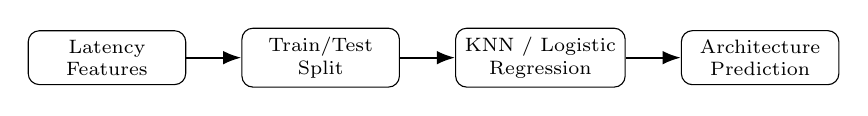
\begin{tikzpicture}[
    node distance=0.7cm,
    block/.style={
        draw,
        rounded corners,
        minimum width=2cm,
        minimum height=0.6cm,
        align=center,
        font=\scriptsize
    },
    arrow/.style={-{Latex}, thick}
]
\node[block] (features) {Latency \\ Features};
\node[block, right=of features] (split) {Train/Test \\ Split};
\node[block, right=of split] (classifier) {KNN / Logistic \\ Regression};
\node[block, right=of classifier] (output) {Architecture \\ Prediction};

\draw[arrow] (features) -- (split);
\draw[arrow] (split) -- (classifier);
\draw[arrow] (classifier) -- (output);
\end{tikzpicture}
}
\caption{Latency-based architecture classification workflow utilized during experiments.}
\label{fig:classification_pipeline}
\end{figure}



\FloatBarrier

% ---------------- RESULTS ----------------
\section{Results}

\subsection{Latency Measurements}

Table~\ref{tab:latency_stats} summarizes the observed latency characteristics across all evaluated architectures.

\begin{table}[H]
\centering
\scriptsize
\caption{Latency Statistics for Different Architectures}
\label{tab:latency_stats}
\begin{tabular}{lccc}
\toprule
Model & Mean (ms) & Std Dev (ms) & P95 (ms) \\
\midrule
ResNet-18 & 42.0168 & 3.9156 & 51.0841 \\
ResNet-50 & 128.7198 & 14.5781 & 159.9856 \\
VGG-16 & 297.7229 & 114.8033 & 604.6216 \\
InceptionV3 & 159.8671 & 75.5069 & 346.9756 \\
\bottomrule
\end{tabular}
\end{table}

\begin{figure}[H]
\centering
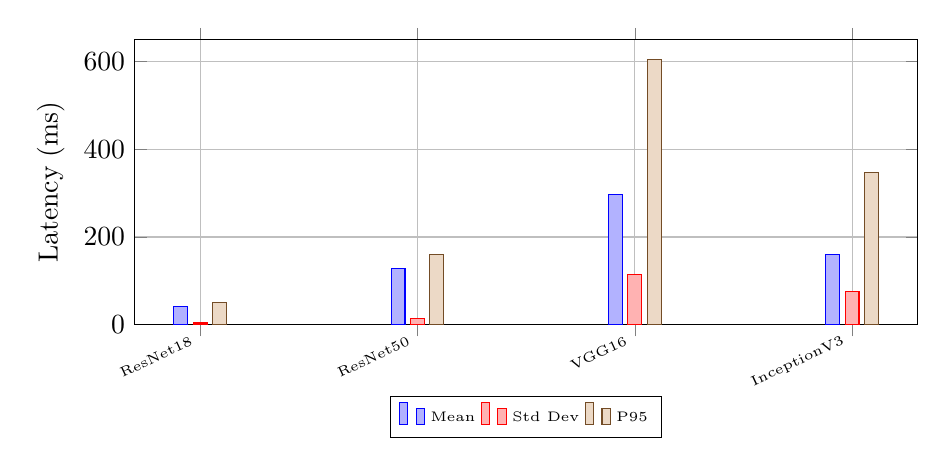
\begin{tikzpicture}
\begin{axis}[
    ybar,
    width=0.95\columnwidth,
    height=5.2cm,
    bar width=5pt,
    ylabel={Latency (ms)},
    symbolic x coords={ResNet18,ResNet50,VGG16,InceptionV3},
    xtick=data,
    x tick label style={rotate=25,anchor=east,font=\tiny},
    ymin=0,
    ymax=650,
    grid=major,
    legend style={
        at={(0.5,-0.25)},
        anchor=north,
        legend columns=3,
        font=\tiny
    }
]
\addplot coordinates {(ResNet18,42.0168) (ResNet50,128.7198) (VGG16,297.7229) (InceptionV3,159.8671)};
\addplot coordinates {(ResNet18,3.9156) (ResNet50,14.5781) (VGG16,114.8033) (InceptionV3,75.5069)};
\addplot coordinates {(ResNet18,51.0841) (ResNet50,159.9856) (VGG16,604.6216) (InceptionV3,346.9756)};
\legend{Mean, Std Dev, P95}
\end{axis}
\end{tikzpicture}
\caption{Latency statistics observed across the evaluated architectures.}
\label{fig:latency_statistics}
\end{figure}

\FloatBarrier

Table~\ref{tab:latency_stats} shows that different neural network architectures exhibit distinct inference latency characteristics. ResNet-18 produced the lowest average latency at 42.0168 ms with relatively low variance, whereas VGG-16 exhibited the highest average latency and the largest latency spread. InceptionV3 and ResNet-50 demonstrated intermediate latency behavior with higher variability compared to ResNet-18.

The P95 latency values further highlight differences in execution behavior across architectures. VGG-16 exhibited the highest tail latency at 604.6216 ms, indicating substantial latency variation during repeated inference execution. InceptionV3 also demonstrated relatively large latency fluctuations compared to ResNet-based architectures.

Figure~\ref{fig:latency_statistics} illustrates the separation between latency distributions across the evaluated architectures. These differences are influenced by architectural properties including network depth, parameter count, branching structure, and computational complexity.

\subsection{Classification Accuracy}

Table~\ref{tab:classification_accuracy} presents the architecture identification performance achieved using latency-derived features.

\begin{table}[H]
\centering
\scriptsize
\caption{Model Identification Accuracy}
\label{tab:classification_accuracy}
\begin{tabular}{lcc}
\toprule
Classifier & Accuracy (\%) & Notes \\
\midrule
KNN & 86.25 & k=5 \\
Logistic Regression & 80.00 &  \\
\bottomrule
\end{tabular}
\end{table}

\begin{figure}[H]
\centering
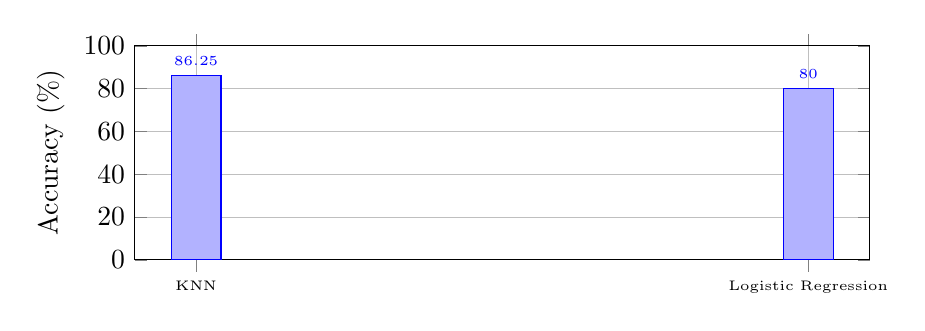
\begin{tikzpicture}
\begin{axis}[
    ybar,
    width=0.9\columnwidth,
    height=4.3cm,
    bar width=18pt,
    ylabel={Accuracy (\%)},
    symbolic x coords={KNN,Logistic Regression},
    xtick=data,
    x tick label style={font=\tiny},
    ymin=0,
    ymax=100,
    grid=major,
    nodes near coords,
    nodes near coords style={font=\tiny}
]
\addplot coordinates {(KNN,86.25) (Logistic Regression,80.00)};
\end{axis}
\end{tikzpicture}
\caption{Architecture identification accuracy using latency-derived statistical features.}
\label{fig:classification_accuracy}
\end{figure}

\begin{table}[H]
\centering
\tiny
\caption{Classification Report for Model Identification}
\label{tab:classification_report}
\begin{tabular}{lccccc}
\toprule
Classifier & Class & Precision & Recall & F1-score & Support \\
\midrule
KNN & ResNet-18 & 1.0000 & 1.0000 & 1.0000 & 20 \\
KNN & ResNet-50 & 0.7917 & 0.9500 & 0.8636 & 20 \\
KNN & VGG-16 & 0.8261 & 0.9500 & 0.8837 & 20 \\
KNN & InceptionV3 & 0.8462 & 0.5500 & 0.6667 & 20 \\
LR & ResNet-18 & 1.0000 & 1.0000 & 1.0000 & 20 \\
LR & ResNet-50 & 0.6250 & 1.0000 & 0.7692 & 20 \\
LR & VGG-16 & 0.8333 & 1.0000 & 0.9091 & 20 \\
LR & InceptionV3 & 1.0000 & 0.2000 & 0.3333 & 20 \\
\bottomrule
\end{tabular}
\end{table}

\FloatBarrier
Table~\ref{tab:classification_accuracy} summarizes the classification accuracy achieved using latency-derived statistical features. The KNN classifier achieved the highest accuracy of 86.25\%, outperforming Logistic Regression, which achieved 80.00\% accuracy. These results indicate that non-linear neighborhood-based classification methods may better capture variations in latency distributions across architectures.

Table~\ref{tab:classification_report} provides a detailed classification report for both classifiers. ResNet-18 achieved perfect precision and recall across both models, indicating highly distinguishable latency characteristics. VGG-16 also demonstrated strong classification performance due to its significantly different latency distribution. InceptionV3 achieved comparatively lower recall values, suggesting partial overlap between its latency characteristics and those of other architectures.

Overall, the results demonstrate that statistical timing features extracted from inference latency contain sufficient discriminative information for neural network architecture fingerprinting in black-box settings.
% ---------------- OPTIONAL ----------------
\subsection{Effect of Query Count}

\begin{table}[H]
\centering
\small
\caption{Accuracy vs Number of Queries}
\label{tab:query_accuracy}
\renewcommand{\arraystretch}{1.25}
\begin{tabular}{cc}
\toprule
Queries & Accuracy (\%) \\
\midrule
1 & 80.0 \\
3 & 85.2 \\
5 & 81.2 \\
10 & 87.5 \\
20 &  \\
\bottomrule
\end{tabular}
\end{table}

\begin{figure}[H]
\centering
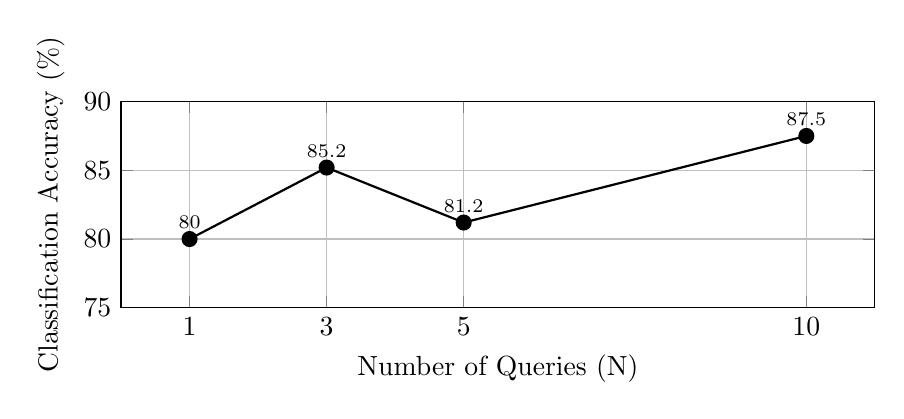
\begin{tikzpicture}
\begin{axis}[
    width=0.92\columnwidth,
    height=4.2cm,
    xlabel={Number of Queries (N)},
    ylabel={Classification Accuracy (\%)},
    xmin=0,
    xmax=11,
    ymin=75,
    ymax=90,
    xtick={1,3,5,10},
    grid=major,
    mark size=2.5pt,
    nodes near coords,
    nodes near coords style={font=\scriptsize,anchor=south}
]
\addplot[
    thick,
    mark=*,
]
coordinates {
(1,80.0)
(3,85.2)
(5,81.2)
(10,87.5)
};
\end{axis}
\end{tikzpicture}
\caption{Query count versus attack success rate for latency-based model fingerprinting.}
\label{fig:accuracy_vs_query_count}
\end{figure}

\FloatBarrier
Looking at Table IV along with Figure 9, it can be observed that increasing the number of queries generally improves classification accuracy. Performance increased from 80.00\% using a single query to 87.5\% when ten queries were utilized. Although the improvement is moderate, the overall trend indicates that additional timing observations improve architecture separability.

One possible explanation for the improved stability at higher query counts is that multiple timing samples help reduce the effect of transient execution noise and system-level timing fluctuations. Minor variations observed at intermediate query counts may be influenced by background processes or small execution inconsistencies during inference.

The results further suggest that repeated timing observations strengthen the ability to distinguish neural network architectures in black-box environments. Overall, the findings indicate that latency patterns, combined with statistical feature extraction, can effectively reveal structural characteristics of deployed neural network systems.
% ---------------- DISCUSSION -------------
% DUMMY PARAGRAPHS (REPLACE LATER) 
\section{Discussion}

The experimental results demonstrate that inference latency contains identifiable architecture-dependent timing patterns. Different neural network architectures exhibited distinct latency distributions due to variations in computational graph topology, execution flow, synchronization behavior, and computational complexity.

The results further indicate that latency variability, in addition to average inference time, contributes significantly to architecture separability. Architectures with deeper or more computationally intensive structures demonstrated broader latency distributions compared to relatively lightweight residual architectures.

Despite the promising results, the experiments were conducted in a controlled CPU-based environment using a limited set of convolutional neural network architectures. Real-world deployment conditions including heterogeneous hardware, background workloads, network jitter, and cloud scheduling behavior may influence latency characteristics and affect fingerprinting performance.

In addition, the current study utilized relatively simple machine learning classifiers and statistical timing descriptors. Future work may investigate more advanced temporal feature extraction techniques, transformer-based architectures, and defensive mechanisms designed to mitigate timing-based information leakage.
% TODO:
% - DAG → latency
% - leakage implications
% - limitations

\FloatBarrier

% ---------------- CONCLUSION ----------------

\section{Conclusion}

This study demonstrated that inference latency can act as a practical side-channel for neural network architecture fingerprinting in black-box deployment environments. Experimental results showed that different CNN architectures produce distinguishable latency distributions due to variations in computational graph structure and execution behavior.

Statistical timing features including mean latency, standard deviation, and tail latency were successfully utilized for architecture classification using lightweight machine learning models. Among the evaluated classifiers, KNN achieved the highest architecture identification accuracy of 86.25\%.

The experiments further demonstrated that increasing the number of timing observations improved classification performance by reducing measurement variability. These findings indicate that inference latency can leak meaningful structural information about deployed neural network models.

Overall, the results highlight the security implications of timing leakage in machine learning systems and demonstrate the feasibility of latency-based neural network fingerprinting in black-box deployment settings.
% TODO:
% - summary
% - key finding
% - future work

\FloatBarrier

\section{Future Work}
Future work may extend the current study by evaluating latency-based architecture fingerprinting across heterogeneous hardware environments including GPUs, edge accelerators, cloud inference servers, and mobile devices. Since hardware-specific optimizations and scheduling behavior can significantly influence inference timing, analyzing cross-platform consistency remains an important direction for improving the generalizability of the proposed methodology.

Further investigation may also incorporate larger and more diverse neural network families including transformer architectures, hybrid models, and quantized networks. Expanding the feature space beyond basic statistical descriptors to include temporal sequences, frequency-domain features, and higher-order timing correlations may improve architecture separability and attack robustness.

Another potential research direction involves studying the impact of real-world deployment conditions such as network jitter, concurrent workloads, caching effects, and asynchronous execution pipelines on timing leakage. Evaluating latency-based fingerprinting in realistic cloud and API-driven inference environments would provide deeper insight into the practical feasibility of side-channel attacks against deployed machine learning systems.

Finally, future research may focus on the development of defensive mechanisms designed to mitigate timing leakage during inference. Techniques such as randomized execution delays, timing obfuscation, workload equalization, and constant-time inference strategies could be explored to reduce architecture-dependent side-channel information while maintaining acceptable inference performance.
% ---------------- REFERENCES ----------------
\begin{thebibliography}{99}

\bibitem{resnet}
K. He, X. Zhang, S. Ren, and J. Sun, ``Deep Residual Learning for Image Recognition,'' in \textit{Proceedings of the IEEE Conference on Computer Vision and Pattern Recognition (CVPR)}, 2016.

\bibitem{vgg}
K. Simonyan and A. Zisserman, ``Very Deep Convolutional Networks for Large-Scale Image Recognition,'' in \textit{International Conference on Learning Representations (ICLR)}, 2015.

\bibitem{inception}
C. Szegedy et al., ``Going Deeper with Convolutions,'' in \textit{Proceedings of the IEEE Conference on Computer Vision and Pattern Recognition (CVPR)}, 2015.

\bibitem{inceptionv3}
C. Szegedy, V. Vanhoucke, S. Ioffe, J. Shlens, and Z. Wojna, ``Rethinking the Inception Architecture for Computer Vision,'' in \textit{Proceedings of the IEEE Conference on Computer Vision and Pattern Recognition (CVPR)}, 2016.

\bibitem{alexnet}
A. Krizhevsky, I. Sutskever, and G. E. Hinton, ``ImageNet Classification with Deep Convolutional Neural Networks,'' in \textit{Advances in Neural Information Processing Systems (NeurIPS)}, 2012.

\bibitem{mobilenet}
A. G. Howard et al., ``MobileNets: Efficient Convolutional Neural Networks for Mobile Vision Applications,'' arXiv preprint arXiv:1704.04861, 2017.

\bibitem{efficientnet}
M. Tan and Q. Le, ``EfficientNet: Rethinking Model Scaling for Convolutional Neural Networks,'' in \textit{International Conference on Machine Learning (ICML)}, 2019.

\bibitem{sidechannel}
P. Kocher, ``Timing Attacks on Implementations of Diffie-Hellman, RSA, DSS, and Other Systems,'' in \textit{Annual International Cryptology Conference (CRYPTO)}, 1996.

\bibitem{cache}
D. Bernstein, ``Cache-Timing Attacks on AES,'' 2005.

\bibitem{mlsecurity}
N. Papernot et al., ``Practical Black-Box Attacks against Machine Learning,'' in \textit{Proceedings of the ACM Asia Conference on Computer and Communications Security}, 2017.

\bibitem{modelstealing}
F. Tramèr et al., ``Stealing Machine Learning Models via Prediction APIs,'' in \textit{USENIX Security Symposium}, 2016.

\bibitem{membership}
R. Shokri et al., ``Membership Inference Attacks against Machine Learning Models,'' in \textit{IEEE Symposium on Security and Privacy}, 2017.

\bibitem{adversarial}
I. J. Goodfellow, J. Shlens, and C. Szegedy, ``Explaining and Harnessing Adversarial Examples,'' in \textit{International Conference on Learning Representations (ICLR)}, 2015.

\bibitem{fingerprinting}
M. Juuti et al., ``PRADA: Protecting Against DNN Model Stealing Attacks,'' in \textit{IEEE European Symposium on Security and Privacy}, 2019.

\bibitem{timingleak}
Y. Batina et al., ``CSI Neural Network: Using Side-Channels to Recover Your Artificial Neural Network Information,'' in \textit{USENIX Security Symposium}, 2019.

\bibitem{survey}
B. Biggio and F. Roli, ``Wild Patterns: Ten Years After the Rise of Adversarial Machine Learning,'' \textit{Pattern Recognition}, vol. 84, pp. 317--331, 2018.

\bibitem{clockwork}
M. Naumov et al., ``Deep Learning Inference in Facebook Data Centers: Characterization, Performance Optimizations and Hardware Implications,'' arXiv preprint arXiv:1811.09886, 2018.

\bibitem{branchynet}
S. Teerapittayanon, B. McDanel, and H. T. Kung, ``BranchyNet: Fast Inference via Early Exiting from Deep Neural Networks,'' in \textit{International Conference on Pattern Recognition (ICPR)}, 2016.

\bibitem{deepsniffer}
L. Yan, Y. Zhou, X. Chen, and J. Xu, ``DeepSniffer: A DNN Model Extraction Framework Based on Learning Architectural Hints,'' in \textit{Proceedings of the ACM International Conference on Architectural Support for Programming Languages and Operating Systems (ASPLOS)}, 2020.

\bibitem{deepcache}
X. Wang et al., ``DeepCache: Principled Cache for Mobile Deep Vision,'' in \textit{Proceedings of the Annual International Conference on Mobile Systems, Applications, and Services (MobiSys)}, 2018.

\bibitem{edgetpu}
N. P. Jouppi et al., ``In-Datacenter Performance Analysis of a Tensor Processing Unit,'' in \textit{Proceedings of the International Symposium on Computer Architecture (ISCA)}, 2017.

\bibitem{gpuperf}
S. Hong and H. Kim, ``An Integrated GPU Power and Performance Model,'' in \textit{Proceedings of the International Symposium on Computer Architecture (ISCA)}, 2010.

\bibitem{mlsys}
C. Zhang et al., ``Understanding Deep Learning System Performance,'' in \textit{Proceedings of the ACM Symposium on Operating Systems Principles (SOSP)}, 2017.

\bibitem{dnnleakage}
M. Hua, Y. Wang, S. Wang, and H. Qian, ``Reverse Engineering Convolutional Neural Networks through Side-Channel Information Leaks,'' in \textit{Design Automation Conference (DAC)}, 2018.

\bibitem{nnextract}
T. Orekondy, B. Schiele, and M. Fritz, ``Knockoff Nets: Stealing Functionality of Black-Box Models,'' in \textit{Proceedings of the IEEE Conference on Computer Vision and Pattern Recognition (CVPR)}, 2019.

\bibitem{modelcopy}
J. Milli et al., ``Model Reconstruction from Model Explanations,'' in \textit{Proceedings of the ACM Conference on Fairness, Accountability, and Transparency (FAT*)}, 2019.

\bibitem{timingml}
J. Wei et al., ``Machine Learning Model Extraction through Hardware Side Channels,'' in \textit{IEEE International Symposium on Hardware Oriented Security and Trust (HOST)}, 2020.

\bibitem{secureinference}
R. Shokri and V. Shmatikov, ``Privacy-Preserving Deep Learning,'' in \textit{Proceedings of the ACM Conference on Computer and Communications Security (CCS)}, 2015.

\bibitem{edgeai}
S. Han et al., ``EIE: Efficient Inference Engine on Compressed Deep Neural Network,'' in \textit{Proceedings of the International Symposium on Computer Architecture (ISCA)}, 2016.

\bibitem{transformers}
A. Vaswani et al., ``Attention Is All You Need,'' in \textit{Advances in Neural Information Processing Systems (NeurIPS)}, 2017.

\bibitem{mldefense}
N. Carlini et al., ``The Secret Sharer: Measuring Unintended Neural Network Memorization \& Extractability,'' in \textit{USENIX Security Symposium}, 2019.
\end{thebibliography}

\end{document}